\documentclass[12pt]{article}

\usepackage[pdftex]{graphicx}
\usepackage{cancel}
\usepackage[margin=4cm]{geometry}
\usepackage[hidelinks]{hyperref}
\usepackage{fancyhdr}
\usepackage{amsmath}
\usepackage{amsfonts}
\usepackage{dirtytalk}
\usepackage{parskip}

\newcommand\tab[1][1cm]{\hspace*{#1}}
\newcommand{\HRule}{\rule{\linewidth}{0.5mm}}
\newcommand{\course}{COMS 474}

\setcounter{secnumdepth}{0} % Disable section/subsection numbering
\hyphenpenalty 10000 % Prevent words from being broken over multiple lines
\exhyphenpenalty 10000 % Prevent words from being broken over multiple lines

% Margins
\topmargin=-0.45in
\evensidemargin=0in
\oddsidemargin=0in
\textwidth=6.5in
\textheight=9.0in
\headsep=0.25in
\title{ \course \\\large Homework 9 }
\author{ Haadi Majeed }
\date{Spring 2022}


\pagestyle{fancy}
\fancyhead{}
\fancyfoot{}
\lhead{\course}
\chead{Haadi Majeed}
\rhead{Page \thepage}

\begin{document}
\maketitle
\pagebreak

% Optional TOC
%\tableofcontents
\pagebreak
\section{Problem 1}
 [26 Points]\\
Suppose that we have a data set with four samples. You calculate the pair-wise distances as\\
\begin{center}
    \begin{tabular}{c c c c c}
        {}    & \{1\} & \{2\} & \{3\} & \{4\} \\
        \{1\} &       & 0.3   & 0.4   & 0.7   \\
        \{2\} & 0.3   &       & 0.5   & 0.8   \\
        \{3\} & 0.4   & 0.5   &       & 0.45  \\
        \{4\} & 0.7   & 0.8   & 0.45  &
    \end{tabular}\\

    \vspace{.2in}


    \emph{dist}$(C_1, C_2) := \underset{a\epsilon C_1, b\epsilon C_2}{min} dist(a,b)$\\
    \emph{dist}$(C_1, C_2) := \underset{a\epsilon C_1, b\epsilon C_2}{max} dist(a,b)$
\end{center}


\subsection{A}
Sketch the dendrogram that results from hierarchically clustering these four samples using complete linkage. Indicate on the plot the height (distance) at which each fusion occurs, as well as the samples corresponding to each leaf in the dendrogram.\\\\
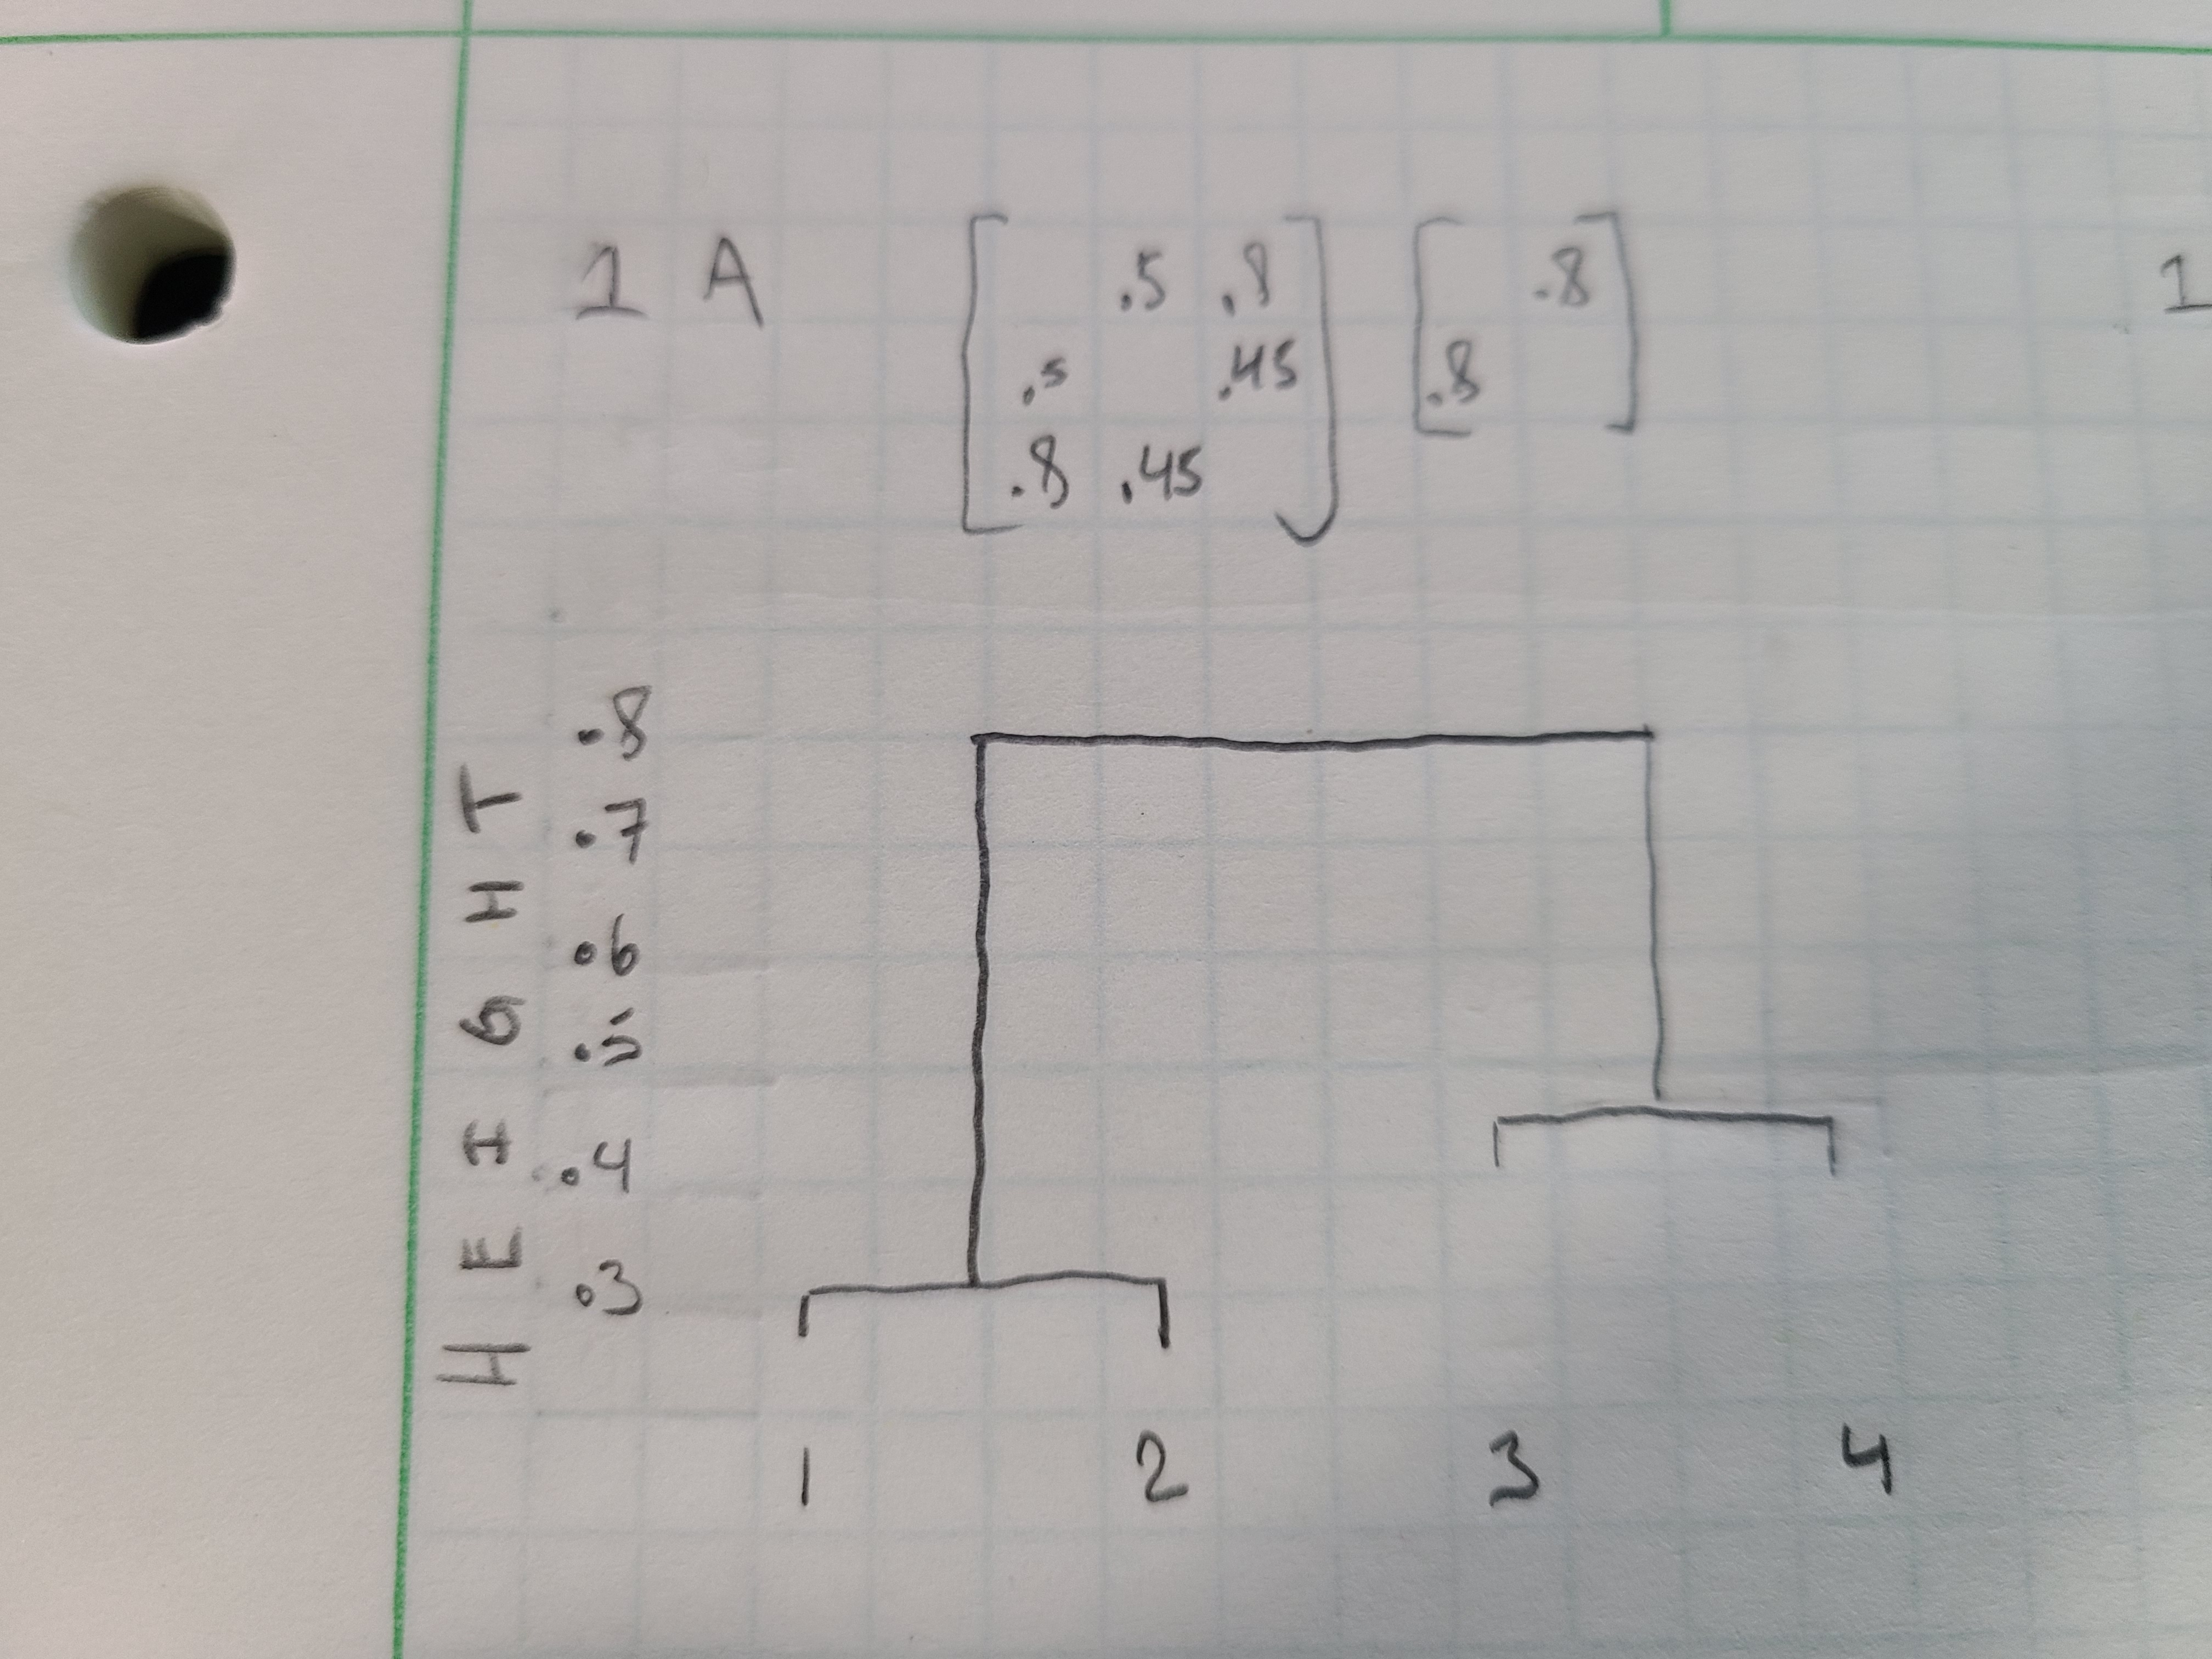
\includegraphics[width=1\textwidth]{p1.a.jpg}

\subsection{B}
Repeat part (a) for single linkage clustering.\\\\
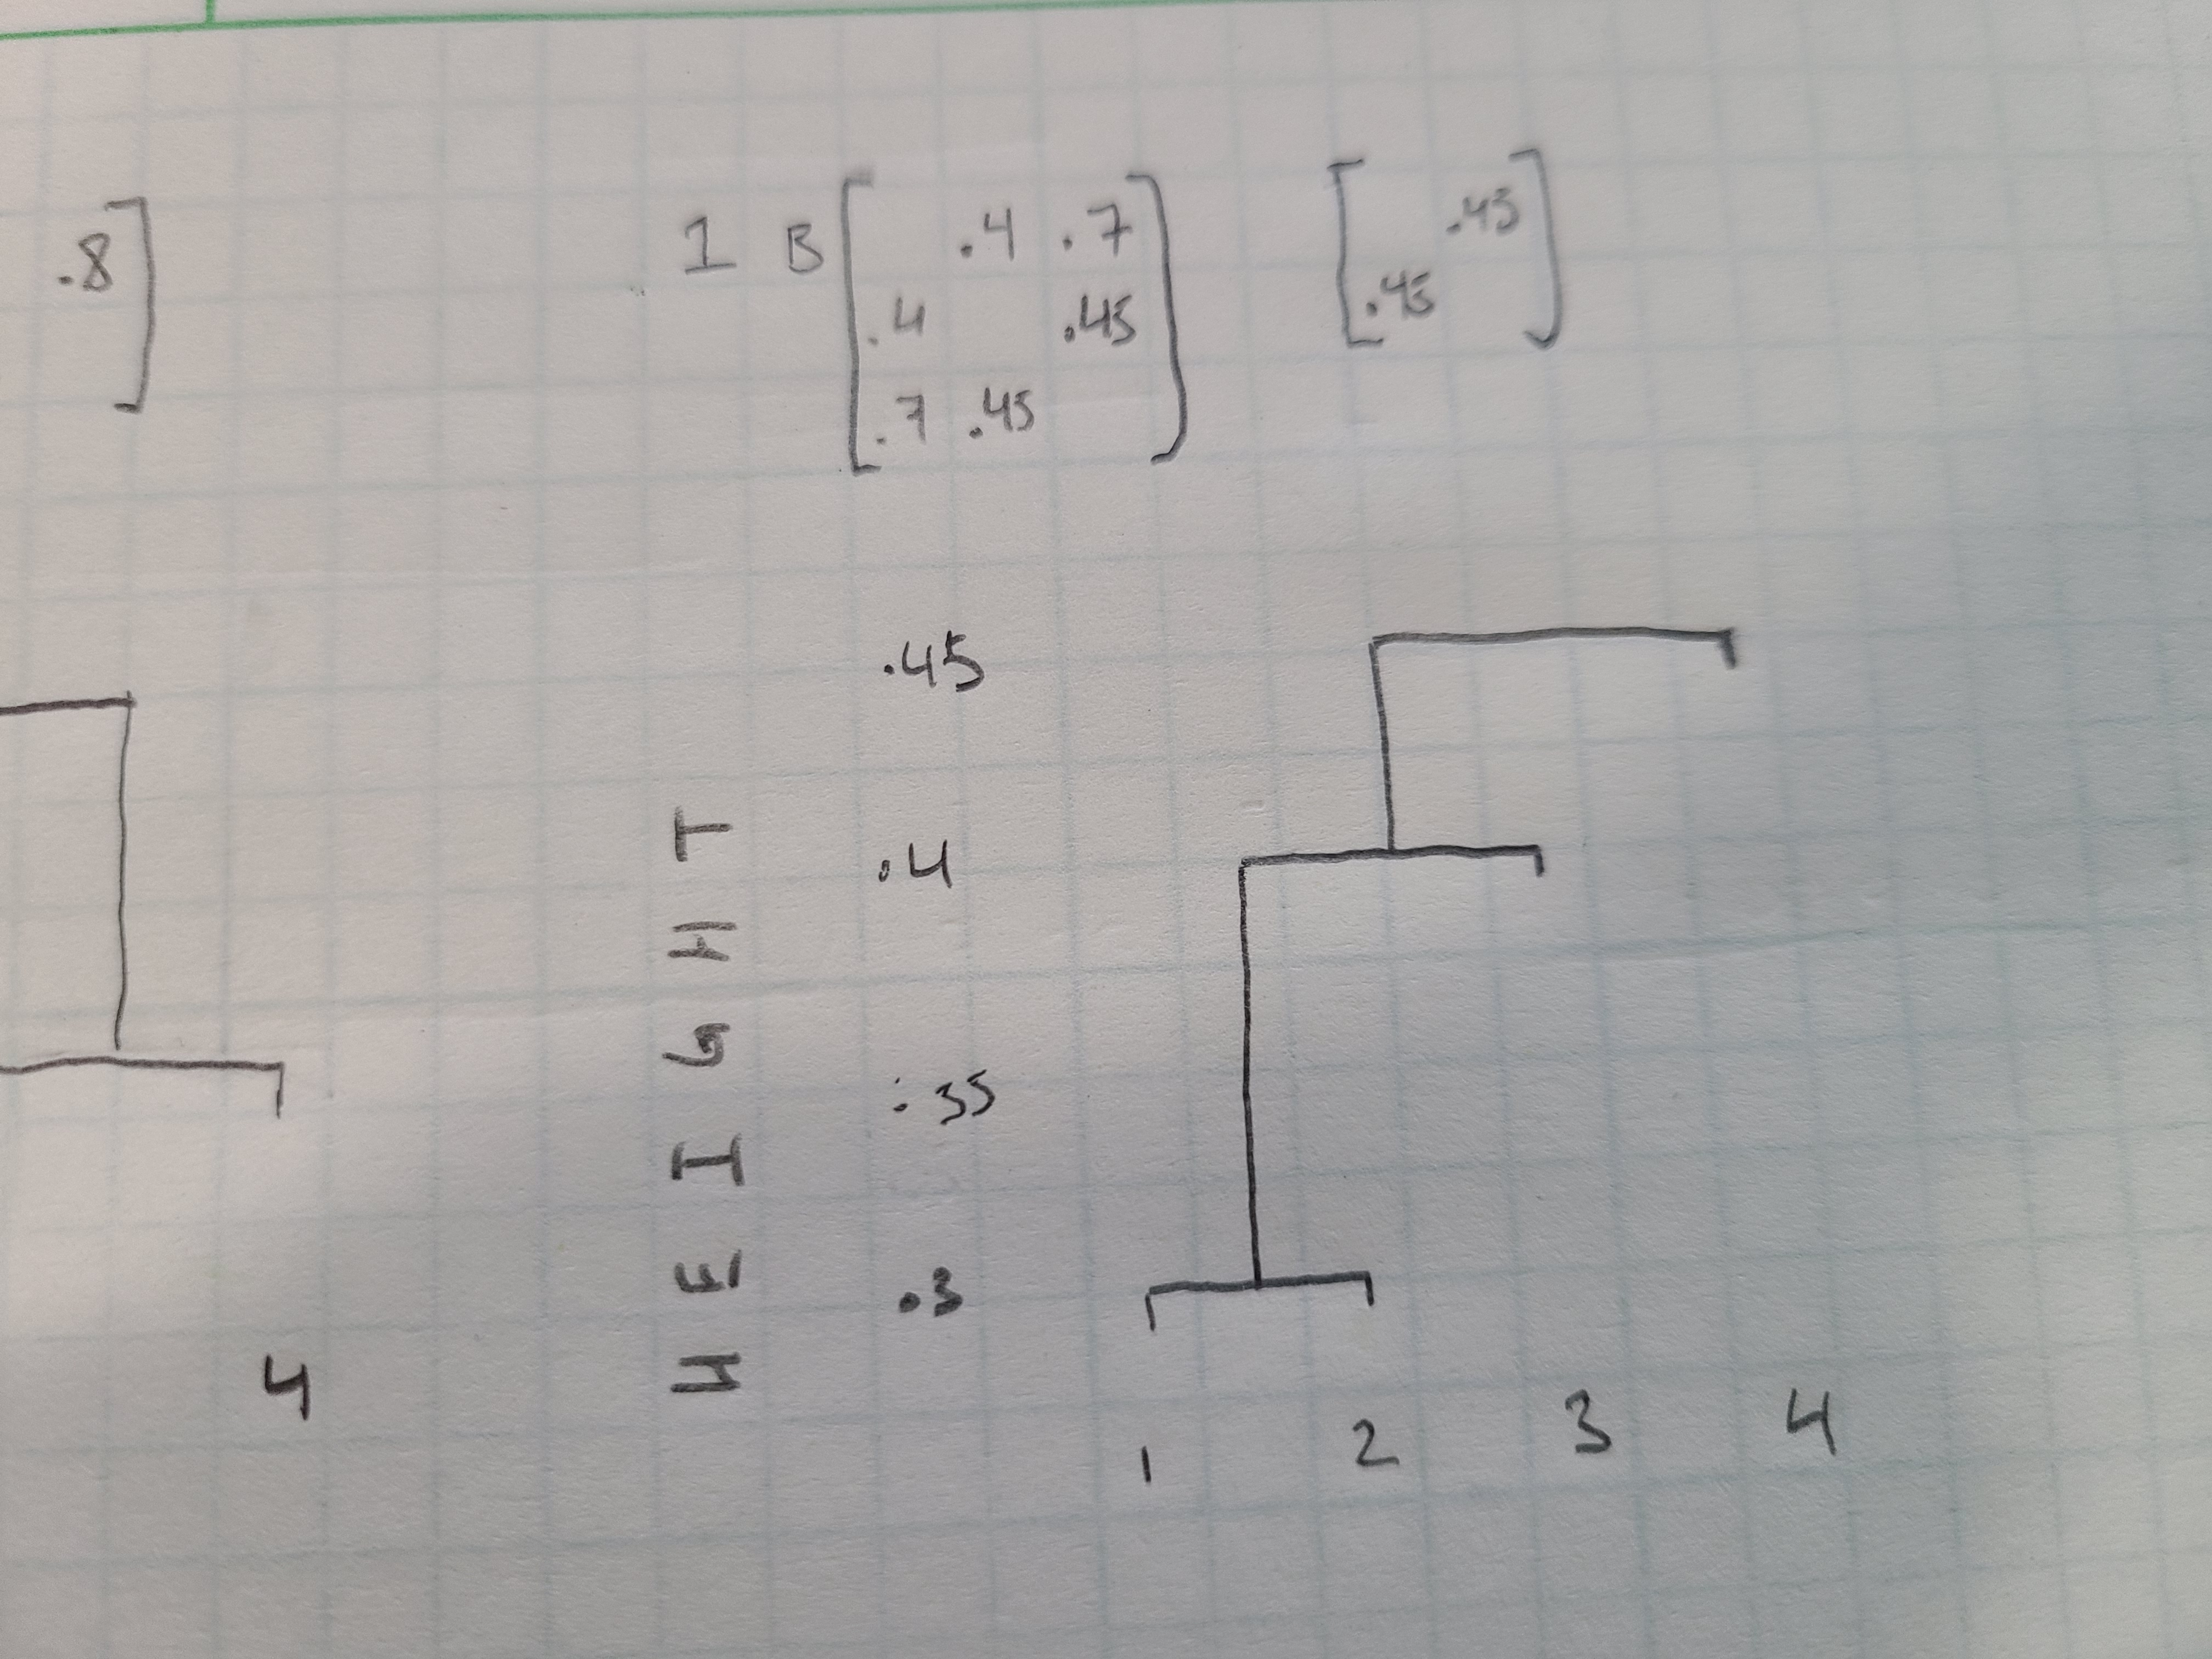
\includegraphics[width=1\textwidth]{p1.b.jpg}


\subsection{C}
Suppose that we cut the dendrogram obtained in (a) such that two clusters result. Which samples are in each cluster?\\\\
The two groups here would be (1, 2) and (3, 4)


\subsection{D}
Suppose that we cut the dendrogram obtained in (b) such that two clusters result. Which samples are in each cluster?\\\\
The two groups would be the following (1, 2, 3) and then (4)


\subsection{E}
Draw a dendrogram that is equivalent to the dendrogram in (a) with a different horizontal arrangement for the samples.\\\\
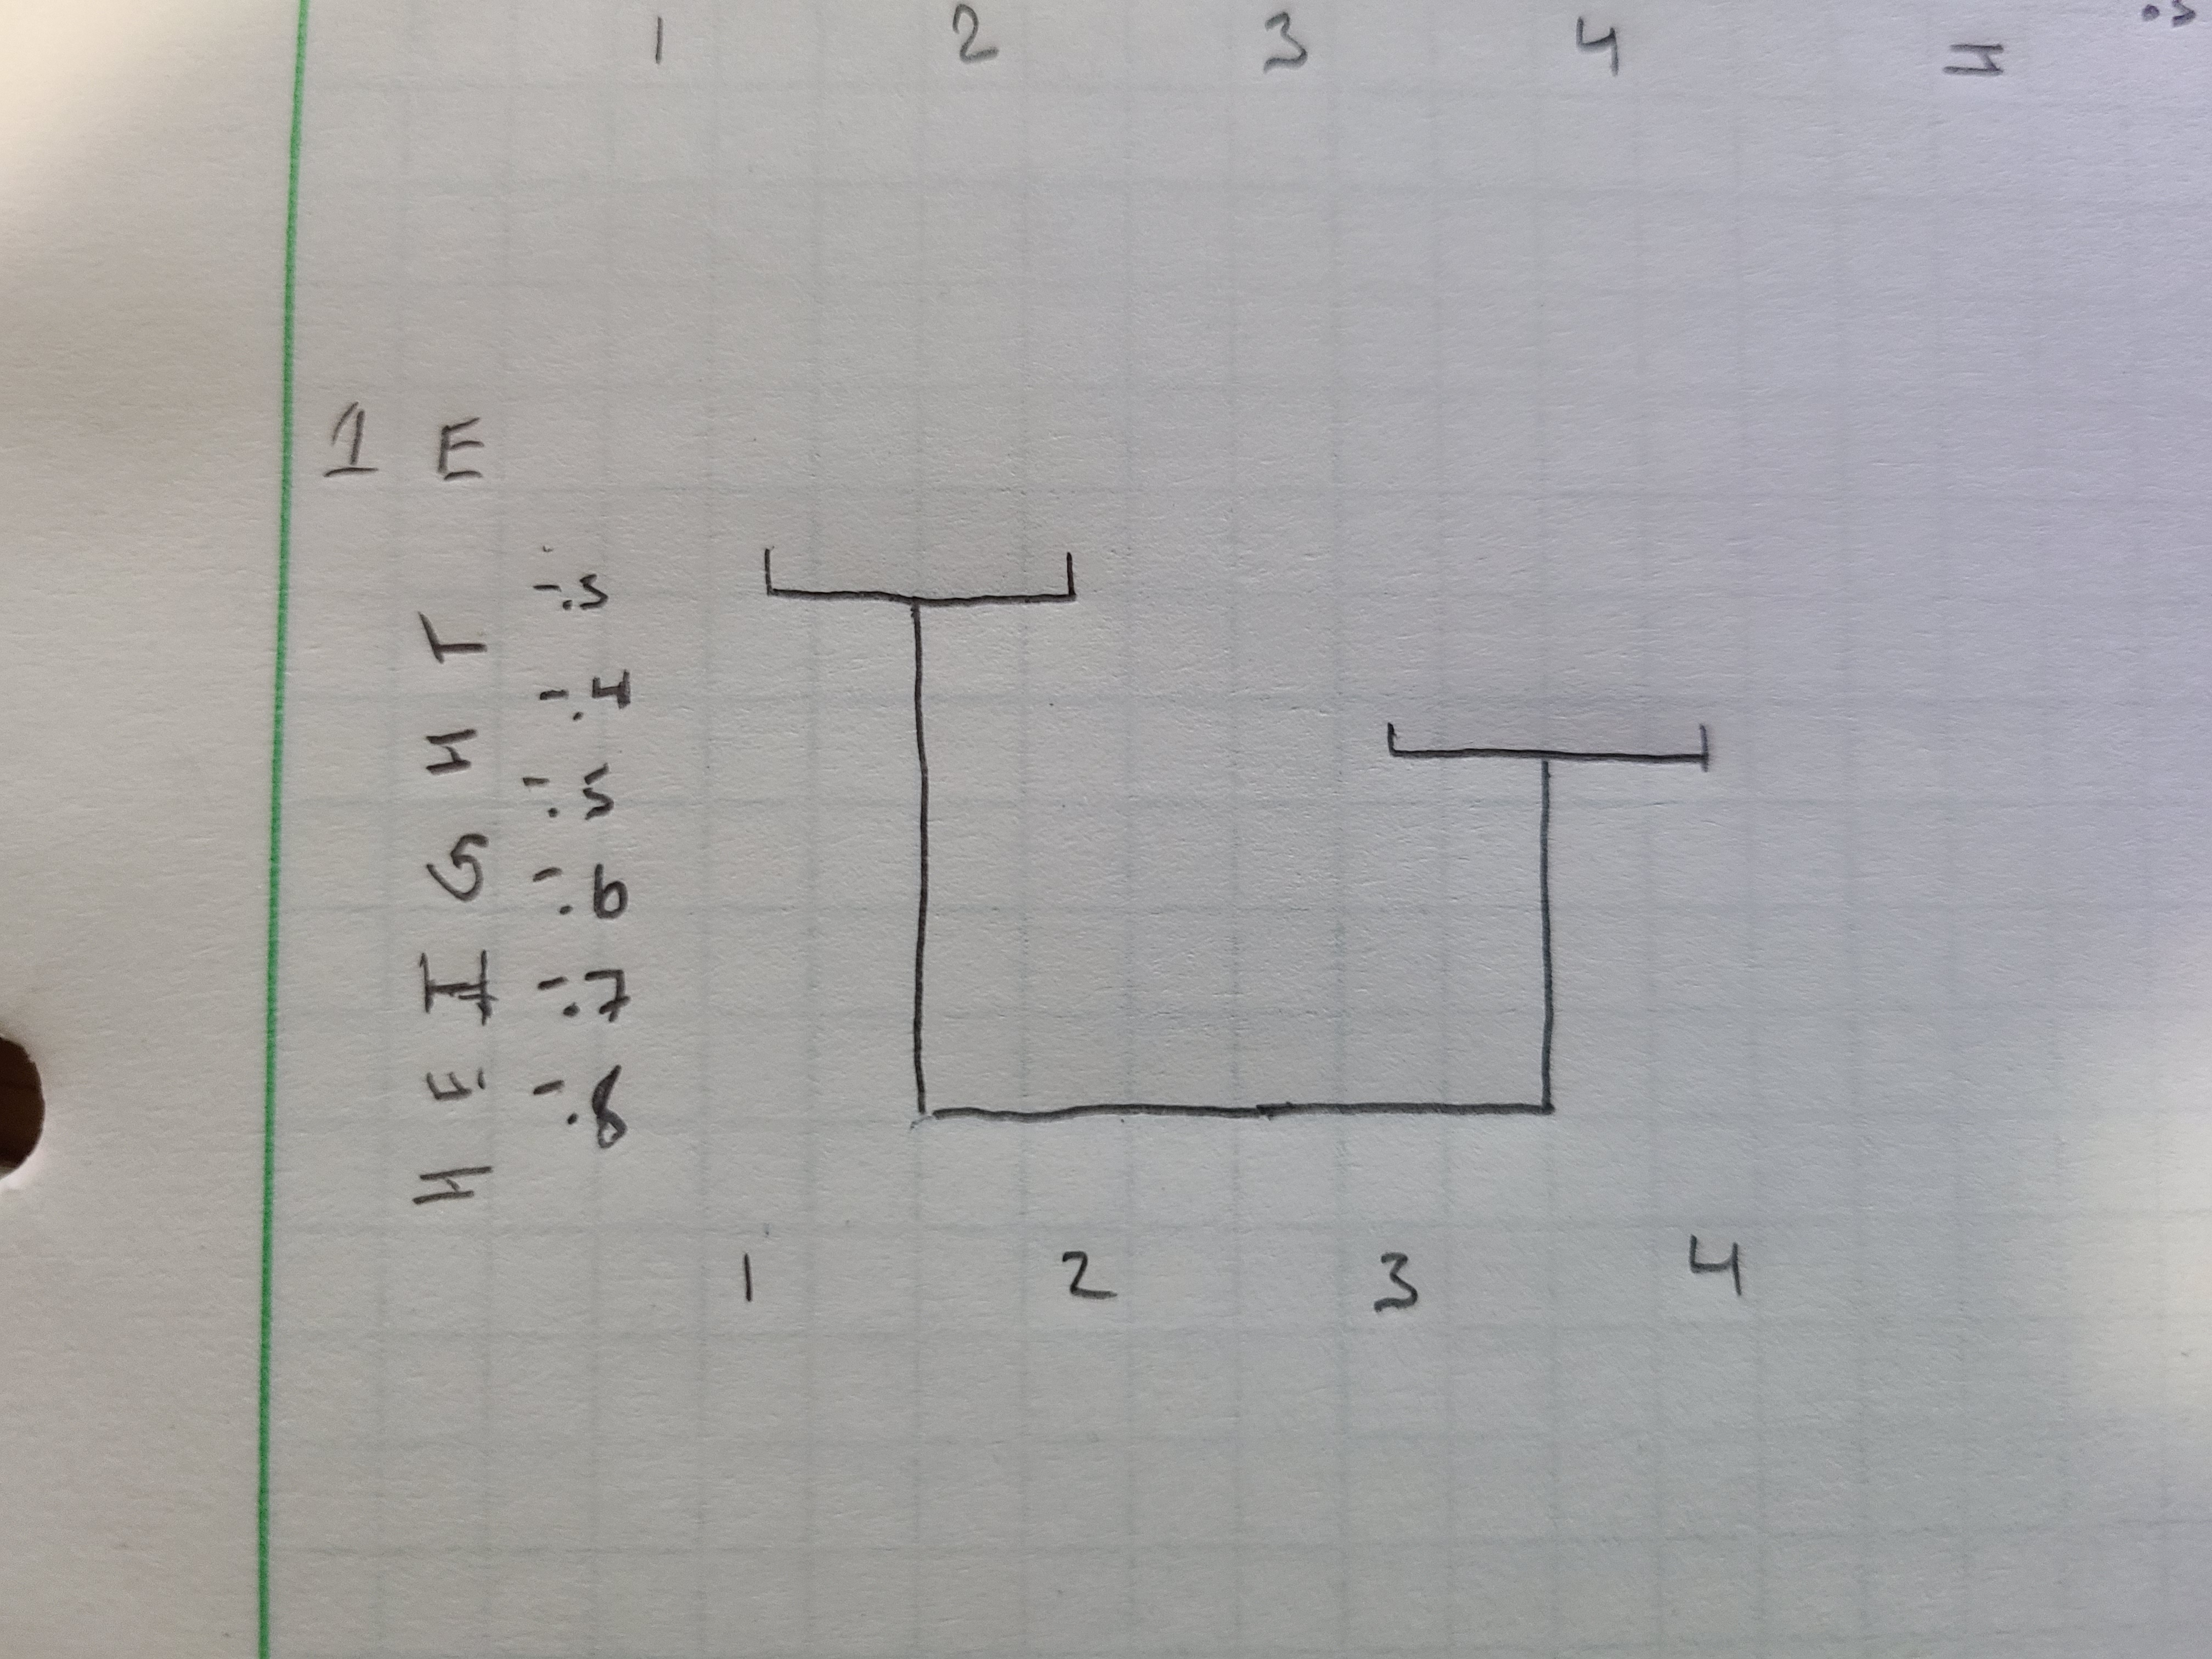
\includegraphics[width=1\textwidth]{p1.e.jpg}



\section{Problem 2}
\subsection{A}
Make a scatter-plot\\\\
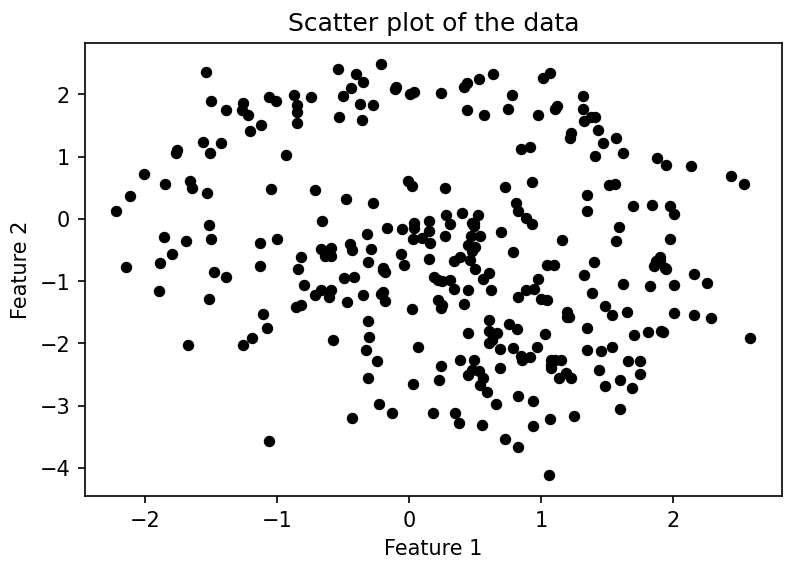
\includegraphics[width=1\textwidth]{p2.a.png}



\subsection{B}
For n\_clusters\=range(1,16), apply K-means clustering. Make a scatter plot for each. You only need to include 3 of them in your homework submission. Select the three pictures whose clusters you think look the best.\\\\
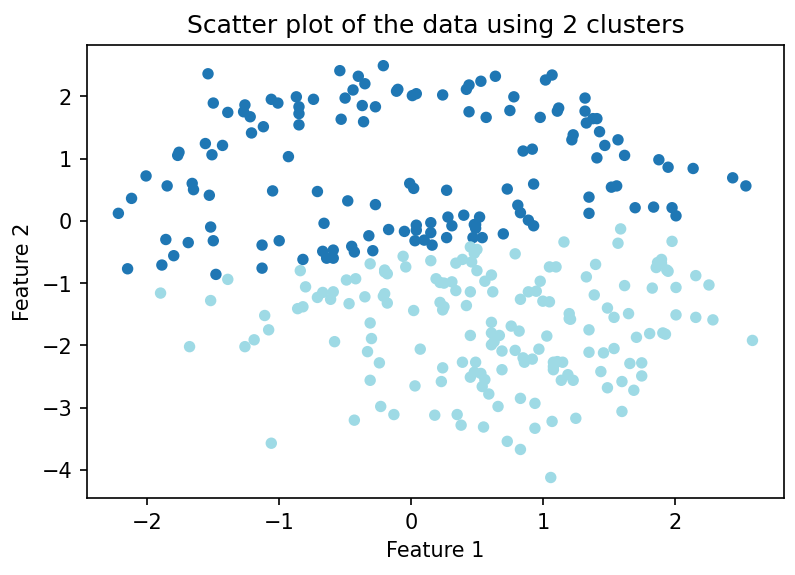
\includegraphics[width=1\textwidth]{p2.b.1.png}\\
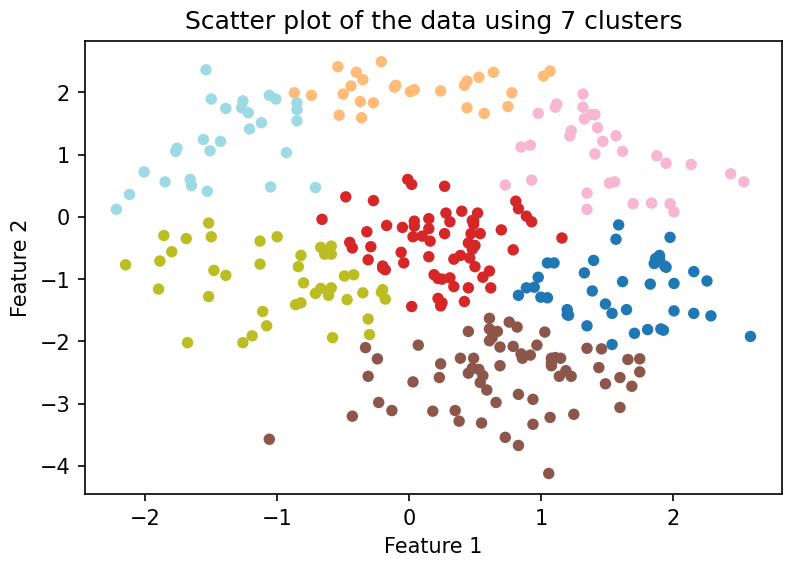
\includegraphics[width=1\textwidth]{p2.b.2.png}\\
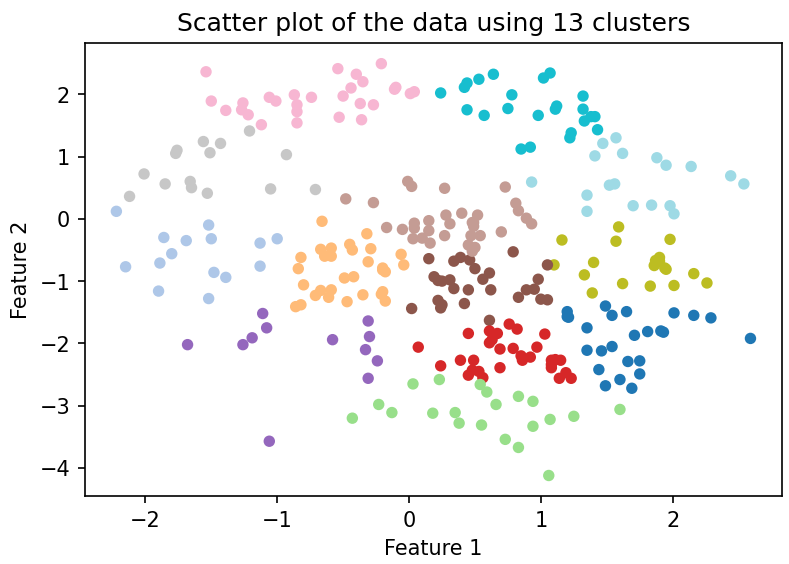
\includegraphics[width=1\textwidth]{p2.b.3.png}




\subsection{C}
For bottom-up hierarchical clustering (aka 'Agglomerative Clustering'), make a dendrogram using 'single' linkage.\\\\
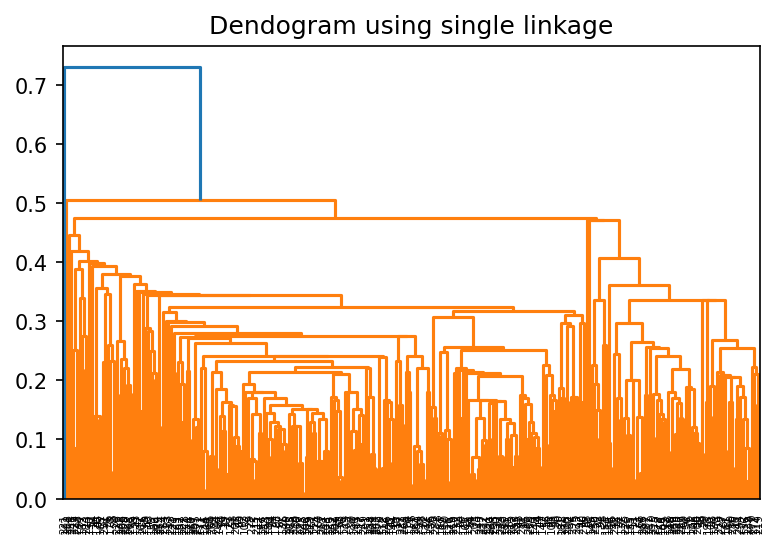
\includegraphics[width=1\textwidth]{p2.c.png}




\subsection{D}
Manually select and report a distance threshold for single linkage. Look for regions in the dendrogram where there are few mergers (eg a big vertical gap in distance threshold between mergers). Use that to make a scatter plot of the data clustered based on that threshold.\\\\
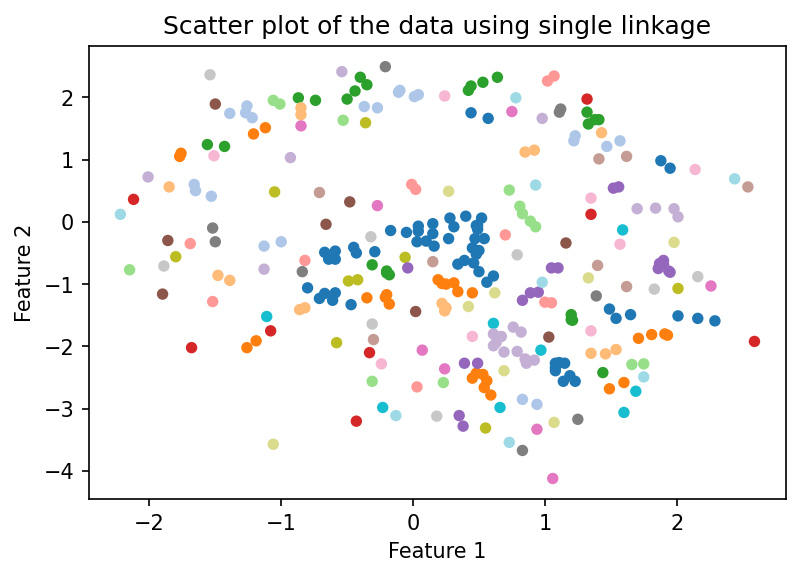
\includegraphics[width=1\textwidth]{p2.d.png}



\subsection{E}
Repeat the previous two steps, using 'average' linkage.\\\\
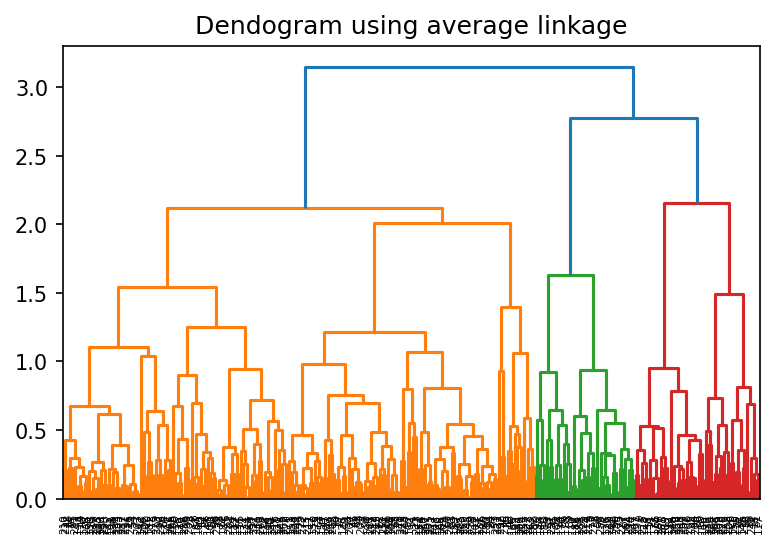
\includegraphics[width=1\textwidth]{p2.e.1.png}
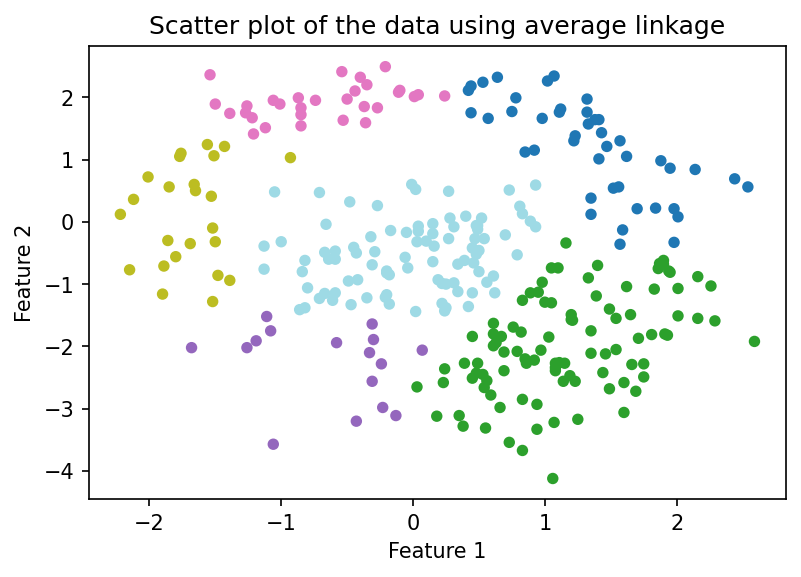
\includegraphics[width=1\textwidth]{p2.e.2.png}




\subsection{F}
Repeat the previous two steps, using 'complete' linkage.\\\\
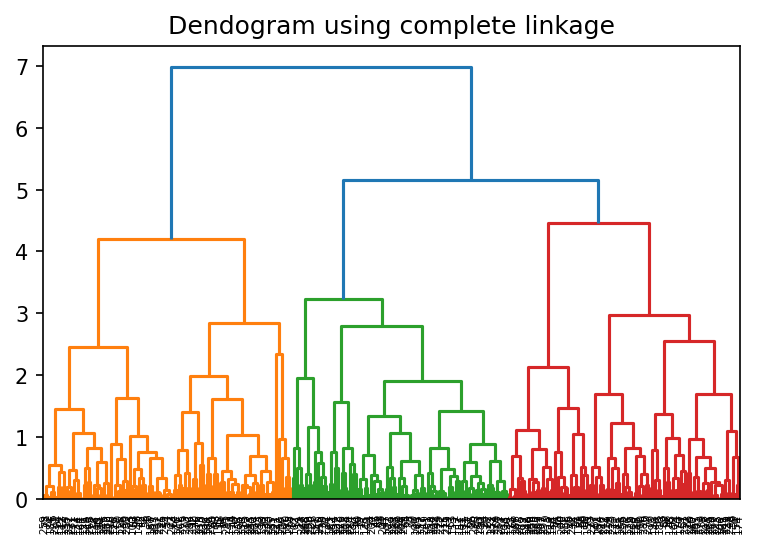
\includegraphics[width=1\textwidth]{p2.f.1.png}
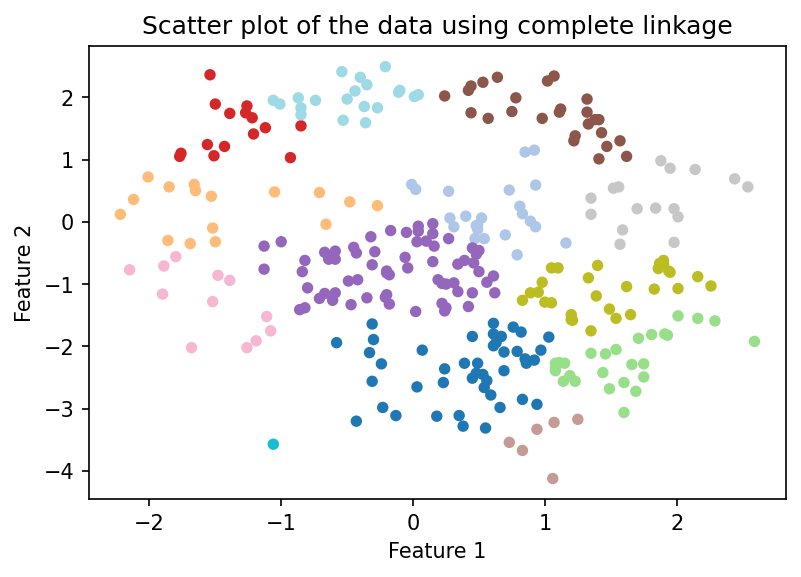
\includegraphics[width=1\textwidth]{p2.f.2.png}




\subsection{G}
In a few sentences for each clustering method (k-means, single linkage aggl., average linkage aggl., and complete linkage aggl.), comment on the clusters found by the methods and how they compared or differed. Which clustering method do you think resulted in the best clusters for this data set and why?\\\\

\subsubsection{K mean}
It just groups with relativity, the results when looking at mid level K values has potential, however too many or too few is just excessive.

\subsubsection{Simple linkage}
The single link dendrogram is terrible, simply put. Its because it goes through each and every single one, one step at a time which makes it look how it does. The data classification is a bit strange, but makes sense that (almost) every single point is a different colour.

\subsubsection{Average linkage}
Average was cool because of how you can almost fully see the boundary lines between each classification. The dendrogram is still a bit unfriendly to look at, however it does convey the message better than simple's did.

\subsubsection{Complete linkage}
Complete linkage groups nicely and matches data similarly to a higher K order and the average, but does better on the dendrogram than the others. It was interesting to see that singular point around (-1, -3) in a classification by itself.


\subsubsection{Overall}
I think overall, simple did the worst in regards to the dendrogram, and this can be very clearly seen in the graph. I would say Complete did the best job classifying the clusters and graphing them since it has a more equal distribution for the data given.

%--/Paper--
\end{document}